\section{Methodology and Project Plan}
\label{sec:methodology}

\subsection{Development Methodology}

Table~\ref{tab:methodologies} compares methodologies against criteria relevant to this project \parencite{sommerville2016}.

\begin{table}[H]
\centering
\begin{tabular}{|l|l|l|l|}
\hline
\textbf{Criteria} & \textbf{Waterfall} & \textbf{Scrum} & \textbf{Iterative Prototyping} \\
\hline
Requirements stability & Requires fixed & Accommodates & Works well when \\
 & requirements upfront & changing requirements & requirements change \\
\hline
Feedback loops & Late feedback after & Sprint reviews every & Continuous feedback \\
 & implementation & 2 to 4 weeks & through prototypes \\
\hline
Risk management & Risks discovered late & Regular risk & Early risk identification \\
 & & reassessment & through prototypes \\
\hline
Solo developer suitability & Moderate & Low (designed for & High \\
 & & teams) & \\
\hline
Research integration & Poor & Moderate & Excellent \\
\hline
\end{tabular}
\caption{Comparison of Development Methodologies}
\label{tab:methodologies}
\end{table}

The project uses iterative prototyping with two-week cycles, drawing on \textcite{boehm1988}'s spiral model (K3, K4, SE8). Each iteration produces a working prototype with a review at cycle's end (SE7). Git with simplified GitFlow (SE12), GitHub Actions CI enforcing 80\% coverage \parencite{fowler2006} (SE6), and ESLint \parencite{eslint2024} handle version control and quality.

\subsection{Requirements Analysis}

Requirements follow MoSCoW prioritisation \parencite{clegg1994} (K9, SE2, SE9).

\subsubsection{Business Requirements}

\begin{enumerate}
    \item \textbf{BR1: Productivity Enhancement}: Reduce time spent on initial PB drafting by generating solid first drafts from minimal input.
    \item \textbf{BR2: Capturing Standards}: Capture company presentation standards through template analysis, reducing reliance on knowledge that lives only in people's heads.
    \item \textbf{BR3: Quality Consistency}: Follow corporate visual identity standards consistently, reducing revision cycles caused by formatting issues.
    \item \textbf{BR4: Data Accuracy}: Financial data in generated PBs should accurately reflect source information.
\end{enumerate}

\subsubsection{Functional Requirements}

Table~\ref{tab:func-req} lists functional requirements by component.

\begin{table}[H]
\centering
\begin{tabular}{|l|l|l|l|}
\hline
\textbf{ID} & \textbf{Component} & \textbf{Requirement} & \textbf{Priority} \\
\hline
FR1 & Template Analyser & Extract slide layouts from reference .pptx files & Must \\
\hline
FR2 & Template Analyser & Identify colour palettes and font specifications & Must \\
\hline
FR3 & Template Analyser & Map placeholder positions and content types & Must \\
\hline
FR4 & Data Retrieval & Fetch company financials from Yahoo Finance API & Must \\
\hline
FR5 & Data Retrieval & Retrieve SEC filings via EDGAR API & Should \\
\hline
FR6 & Data Retrieval & Perform web searches for company news & Should \\
\hline
FR7 & Content Planner & Generate slide-by-slide content specifications & Must \\
\hline
FR8 & Content Planner & Adapt content structure to PB type & Must \\
\hline
FR9 & Content Planner & Maintain narrative coherence across slides & Should \\
\hline
FR10 & Slide Builder & Assemble slides matching template layouts & Must \\
\hline
FR11 & Slide Builder & Populate placeholders with generated content & Must \\
\hline
FR12 & Slide Builder & Generate charts from financial data & Could \\
\hline
FR13 & Orchestration & Coordinate multi-step generation workflow & Must \\
\hline
FR14 & Orchestration & Handle API failures gracefully & Should \\
\hline
FR15 & RAG Search & Query precedent material repository & Could \\
\hline
\end{tabular}
\caption{Functional Requirements Specification}
\label{tab:func-req}
\end{table}

\subsubsection{Non-Functional Requirements}

\begin{table}[H]
\centering
\begin{tabular}{|l|l|l|l|}
\hline
\textbf{ID} & \textbf{Category} & \textbf{Requirement} & \textbf{Acceptance Criterion} \\
\hline
NFR1 & Performance & System generates complete PB draft & Within 5 minutes of input submission \\
\hline
NFR2 & Performance & API response handling & Timeout after 30s with graceful fallback \\
\hline
NFR3 & Reliability & System availability during demonstration & 95\% uptime during evaluation period \\
\hline
NFR4 & Usability & Input specification interface & Requires no technical expertise to operate \\
\hline
NFR5 & Maintainability & Codebase documentation & All public functions documented \\
\hline
NFR6 & Security & API credential management & No credentials in source code \\
\hline
NFR7 & Security & Input validation & All user inputs sanitised before processing \\
\hline
NFR8 & Compatibility & Output format & Valid .pptx files openable in PowerPoint \\
\hline
\end{tabular}
\caption{Non-Functional Requirements Specification}
\label{tab:nfr}
\end{table}

\subsection{Technology Stack}

\subsubsection{Programming Language and Framework}

Table~\ref{tab:lang-comparison} compares language options (K8, SE12).

\begin{table}[H]
\centering
\begin{tabular}{|l|l|l|l|}
\hline
\textbf{Criteria} & \textbf{TypeScript/Node.js} & \textbf{Python} & \textbf{Java} \\
\hline
Benefits & Type safety, same language & Best AI/ML libraries, & Strong typing, \\
 & frontend and backend, & mature PowerPoint & enterprise support \\
 & native async & library (python-pptx) & \\
\hline
Risks & AI/ML ecosystem less & Two languages needed & Verbose code, \\
 & mature than Python & (Python backend + & slower development \\
 & & JS frontend) & \\
\hline
PowerPoint & PptxGenJS (actively & python-pptx (mature, & Apache POI \\
manipulation & maintained, typed) & well-documented) & (verbose API) \\
\hline
Full-stack & Single language across & Requires separate & Requires separate \\
coherence & all three apps & frontend framework & frontend framework \\
\hline
\end{tabular}
\caption{Programming Language Comparison}
\label{tab:lang-comparison}
\end{table}

The deciding factor was using one language everywhere. The \texttt{shared-types} package defines data models once and shares them across all three apps. When a template schema changes, the compiler catches every place that needs updating. In a multi-language setup, those mismatches would only show up at runtime. Express.js handles the backend.

\subsubsection{AI and LLM Integration}

Table~\ref{tab:llm-comparison} compares the LLM options considered.

\begin{table}[H]
\centering
\begin{tabular}{|l|l|l|l|}
\hline
\textbf{Criteria} & \textbf{GPT-4/GPT-4o} & \textbf{Claude 3.5} & \textbf{Gemini 2.0 Flash} \\
\hline
Benefits & Best structured output, & Largest context window & Massive context (1M \\
 & mature SDK, native JSON & (200K), strong reasoning & tokens), fast inference \\
\hline
Risks & Higher cost per token & Newer agent tooling & Less mature structured \\
 & & & output \\
\hline
Structured output & Excellent (native JSON) & Good & Good \\
\hline
Cost (student budget) & Moderate (tiered pricing) & Moderate & Very affordable \\
\hline
\end{tabular}
\caption{Large Language Model Comparison}
\label{tab:llm-comparison}
\end{table}

GPT-4o was chosen for its structured output reliability. OpenAI's native JSON mode produces well-formed responses more consistently than alternatives, which matters when output feeds directly into a Zod validation pipeline. GPT-4o-mini handles the lighter AI chat feature at lower cost. Swapping models later requires changing only the API call.

\subsubsection{Data Sources and APIs}

Table~\ref{tab:data-sources} summarises data sources.

\begin{table}[H]
\centering
\begin{tabular}{|l|l|l|l|}
\hline
\textbf{Source} & \textbf{Benefits} & \textbf{Risks} & \textbf{Access} \\
\hline
Yahoo Finance & Free, comprehensive & Unofficial API may & yahoo-finance2 \\
 & financial data & change without notice & npm package \\
\hline
SEC EDGAR & Official regulatory & US companies only, & REST API \\
 & filings, reliable, free & complex document parsing & (10 req/s) \\
\hline
Web Search & Current news, market & Cost per query & SerpAPI or similar \\
 & commentary & & \\
\hline
\end{tabular}
\caption{External Data Sources}
\label{tab:data-sources}
\end{table}

\subsubsection{Frontend and Deployment}

Next.js handles the web frontend for PB creation and management.

\begin{table}[H]
\centering
\begin{tabular}{|l|l|l|l|}
\hline
\textbf{Criteria} & \textbf{Vercel + Render} & \textbf{AWS} & \textbf{Self-hosted} \\
\hline
Benefits & Zero config, auto deploy, & Full control, & Complete control, \\
 & free tiers for POC & scalable & no vendor lock-in \\
\hline
Risks & Vendor lock-in, cold starts & Complex setup, cost & Maintenance burden \\
\hline
Cost for POC & Free tier sufficient & May incur charges & Server costs \\
\hline
\end{tabular}
\caption{Deployment Platform Comparison}
\label{tab:deploy}
\end{table}

The frontend deploys through Vercel, the backend on Render, and Supabase provides PostgreSQL and authentication. Figure~\ref{fig:tech-architecture} shows how the chosen technologies map to the system's components.

\begin{figure}[H]
\centering
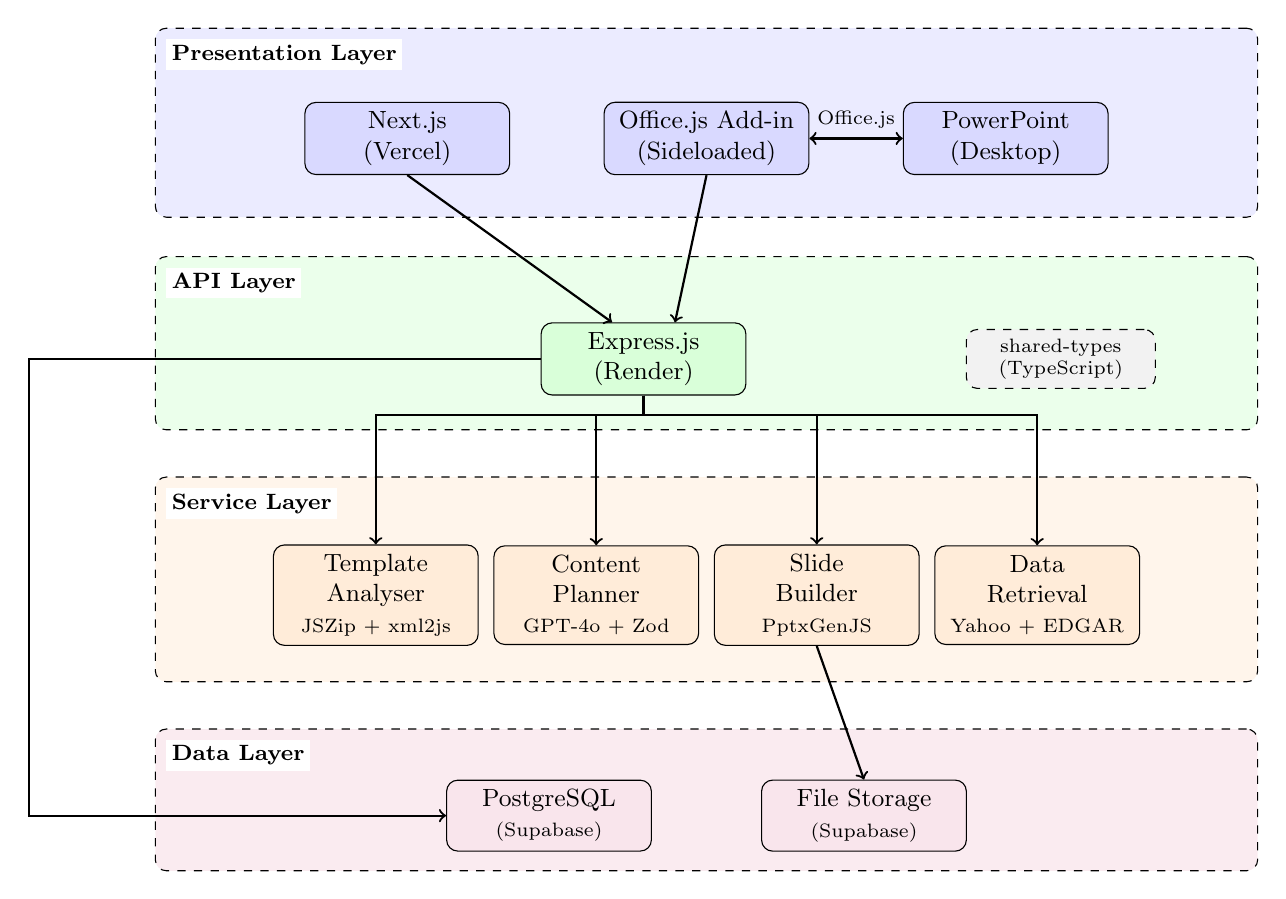
\begin{tikzpicture}[
  box/.style={draw, rounded corners, minimum width=2.6cm, minimum height=0.9cm, align=center, font=\small},
  arr/.style={->, thick},
  darr/.style={<->, thick},
  layer/.style={draw, dashed, rounded corners, inner sep=12pt, fill=#1, fill opacity=0.08, text opacity=1},
  lbl/.style={font=\footnotesize\bfseries, fill=white, inner sep=2pt},
]

% --- Presentation Layer ---
\node[layer=blue, minimum width=14cm, minimum height=2.4cm] (pres) at (0, 6) {};
\node[lbl, anchor=north west] at ([xshift=4pt, yshift=-4pt]pres.north west) {Presentation Layer};

\node[box, fill=blue!15] (web) at (-3.8, 5.8) {Next.js\\(Vercel)};
\node[box, fill=blue!15] (addin) at (0, 5.8) {Office.js Add-in\\(Sideloaded)};
\node[box, fill=blue!15] (ppt) at (3.8, 5.8) {PowerPoint\\(Desktop)};

\draw[darr] (addin) -- node[above, font=\scriptsize] {Office.js} (ppt);

% --- API Layer ---
\node[layer=green, minimum width=14cm, minimum height=2.2cm] (apil) at (0, 3.2) {};
\node[lbl, anchor=north west] at ([xshift=4pt, yshift=-4pt]apil.north west) {API Layer};

\node[box, fill=green!15] (api) at (-0.8, 3) {Express.js\\(Render)};
\node[draw, dashed, rounded corners, minimum width=2.4cm, minimum height=0.7cm, fill=gray!10, font=\scriptsize, align=center] (types) at (4.5, 3) {shared-types\\(TypeScript)};

\draw[arr] (web.south) -- ([xshift=-0.4cm]api.north);
\draw[arr] (addin.south) -- ([xshift=0.4cm]api.north);

% --- Service Layer ---
\node[layer=orange, minimum width=14cm, minimum height=2.6cm] (svcl) at (0, 0.2) {};
\node[lbl, anchor=north west] at ([xshift=4pt, yshift=-4pt]svcl.north west) {Service Layer};

\node[box, fill=orange!15] (ta) at (-4.2, 0) {Template\\Analyser\\{\scriptsize JSZip + xml2js}};
\node[box, fill=orange!15] (cp) at (-1.4, 0) {Content\\Planner\\{\scriptsize GPT-4o + Zod}};
\node[box, fill=orange!15] (sb) at (1.4, 0) {Slide\\Builder\\{\scriptsize PptxGenJS}};
\node[box, fill=orange!15] (dr) at (4.2, 0) {Data\\Retrieval\\{\scriptsize Yahoo + EDGAR}};

\draw[arr] (api.south) -- ++(0,-0.25) -| (ta.north);
\draw[arr] (api.south) -- ++(0,-0.25) -| (cp.north);
\draw[arr] (api.south) -- ++(0,-0.25) -| (sb.north);
\draw[arr] (api.south) -- ++(0,-0.25) -| (dr.north);

% --- Data Layer ---
\node[layer=purple, minimum width=14cm, minimum height=1.8cm] (datal) at (0, -2.6) {};
\node[lbl, anchor=north west] at ([xshift=4pt, yshift=-4pt]datal.north west) {Data Layer};

\node[box, fill=purple!10] (db) at (-2, -2.8) {PostgreSQL\\{\scriptsize (Supabase)}};
\node[box, fill=purple!10] (storage) at (2, -2.8) {File Storage\\{\scriptsize (Supabase)}};

% Route api->db down the far left, outside all boxes
\draw[arr] (api.west) -- ++(-6.5,0) |- (db.west);
% Route sb->storage straight down
\draw[arr] (sb.south) -- (storage.north);

\end{tikzpicture}
\caption{Technology architecture showing how chosen technologies map to system components across four layers. Arrows indicate data flow direction.}
\label{fig:tech-architecture}
\end{figure}

\subsection{Reproducibility}

Dependencies are pinned via \texttt{package-lock.json}, LLM temperature is set to zero for evaluation runs, and each run is tied to a specific Git commit. GPT-4o does not guarantee identical outputs at temperature zero \parencite{runeson2012}, so Zod validation ensures structural consistency.

\subsection{Evaluation Methodology}

The evaluation follows the Goal-Question-Metric (GQM) approach \parencite{basili1994}, keeping every metric tied to a specific project goal. The goal: determine whether the system produces usable first drafts faster than manual creation while matching template formatting.

\begin{table}[H]
\centering
\begin{tabular}{|l|l|l|}
\hline
\textbf{Question} & \textbf{Metric} & \textbf{Target} \\
\hline
How fast does the system & Generation time per & Under 300 seconds \\
generate a deck? & 10-slide deck & for a complete draft \\
\hline
Does the output match & Colour and font & Exact colour and \\
the reference template? & comparison (programmatic) & font match \\
\hline
Is the financial data & Comparison against & 100\% match on market cap, \\
correct? & source API responses & revenue, and share price \\
\hline
Does the content follow & Rubric-based assessment & Correct section ordering \\
IB conventions? & of narrative structure & across 3 PB types \\
\hline
\end{tabular}
\caption{GQM Evaluation Framework}
\label{tab:gqm}
\end{table}

Targets were fixed before evaluation began \parencite{wohlin2012}. Outputs are compared against generic tools (Gamma, Beautiful.ai) and estimated manual creation time. An informal usability evaluation with four junior analysts (P1--P4) provides qualitative feedback.

\subsection{Project Plan}

The project runs for thirteen weeks (K10). Figure~\ref{fig:gantt} shows the schedule, and Table~\ref{tab:milestones} lists milestones. Dates are targets. If a milestone slips, `Could have' requirements are dropped first.

\begin{figure}[H]
\centering
\resizebox{\textwidth}{!}{%
\begin{ganttchart}[
    hgrid,
    vgrid={*{12}{draw=gray!30}},
    x unit=1.1cm,
    y unit chart=0.45cm,
    y unit title=0.55cm,
    title height=1,
    bar/.style={fill=blue!30, draw=blue!50},
    group/.style={draw=black, fill=blue!60},
    group left shift=0,
    group right shift=0,
    group height=0.4,
    group peaks tip position=0,
    bar height=0.5,
    bar label font=\small,
    group label font=\small\bfseries,
    title label font=\normalsize\bfseries,
    milestone label font=\small\itshape,
]{1}{13}
\gantttitle[title label node/.append style={anchor=east, left=-3pt}]{}{0}
\gantttitle{Jan}{2}
\gantttitle{Feb}{4}
\gantttitle{Mar}{4}
\gantttitle{Apr}{3} \\
\gantttitle[title label node/.append style={anchor=east, xshift=-2pt}]{Week}{0}
\gantttitlelist{1,...,13}{1} \\
%
% 1. Introduction and Methodology
\ganttgroup{Introduction \& Methodology}{1}{2} \\
\ganttbar{Project scope and objectives}{1}{2} \\
\ganttbar{Methodology comparison}{1}{2} \\
%
% 2. Literature Review
\ganttgroup{Literature Review}{2}{4} \\
\ganttbar{AI tools in investment banking}{2}{3} \\
\ganttbar{LLM structured output patterns}{2}{3} \\
\ganttbar{PowerPoint automation approaches}{3}{4} \\
%
% 3. Research and Design
\ganttgroup{Research \& Design}{3}{6} \\
\ganttbar{System architecture and API contracts}{3}{4} \\
\ganttbar{Database schema and data models}{4}{5} \\
\ganttbar{Technology evaluation (LLMs, APIs, deployment)}{3}{6} \\
%
% 4. Implementation
\ganttgroup{Implementation}{5}{10} \\
\ganttbar{Express backend and service pipeline}{5}{6} \\
\ganttbar{Template analyser (JSZip, xml2js)}{5}{7} \\
\ganttbar{Data retrieval (Yahoo Finance, SEC EDGAR)}{6}{7} \\
\ganttbar{Content planner (GPT-4o integration)}{6}{8} \\
\ganttbar{Slide builder (PptxGenJS)}{7}{8} \\
\ganttbar{Next.js web application}{7}{9} \\
\ganttbar{PowerPoint add-in (Office.js)}{8}{10} \\
\ganttbar{Slide preview pipeline (LibreOffice)}{9}{10} \\
%
% 5. Evaluation
\ganttgroup{Evaluation}{9}{11} \\
\ganttbar{Unit and integration tests (Vitest)}{9}{10} \\
\ganttbar{E2E tests (Cypress)}{9}{10} \\
\ganttbar{Generation evaluation runs}{10}{11} \\
\ganttbar{Usability evaluation with analysts}{10}{11} \\
%
% 6. Finalisation
\ganttgroup{Finalisation}{11}{13} \\
\ganttbar{Report writing and revisions}{11}{12} \\
\ganttbar{Proofreading and formatting}{12}{13} \\
\ganttmilestone{Submission}{13}
\end{ganttchart}%
}
\caption{Project Gantt Chart (weeks 1 to 13, January to April 2026)}
\label{fig:gantt}
\end{figure}

\begin{table}[H]
\centering
\begin{tabular}{|l|l|l|l|}
\hline
\textbf{Phase} & \textbf{Date} & \textbf{Milestone} & \textbf{Deliverables} \\
\hline
1 & 19 Jan & Project Initiation & Repository setup, dev environment configured \\
\hline
2 & 31 Jan & Initial Chapters & Introduction, Scope, Methodology complete \\
\hline
3 & 21 Feb & Literature Review & Literature review chapter complete \\
\hline
4 & 28 Feb & Design Complete & Architecture diagrams, API specs, data models \\
\hline
5 & 14 Mar & Core Components & Template analyser and data retrieval functional \\
\hline
6 & 28 Mar & MVP Complete & End-to-end generation pipeline operational \\
\hline
7 & 4 Apr & Testing Complete & Tests passing, evaluation data collected \\
\hline
8 & 11 Apr & Evaluation Complete & Results analysis and evaluation chapter written \\
\hline
9 & 18 Apr & Document Finalised & All chapters complete, proofread, formatted \\
\hline
10 & 20 Apr & Submission & Final report submitted via QMPlus \\
\hline
\end{tabular}
\caption{Project Milestones and Deliverables}
\label{tab:milestones}
\end{table}

\subsection{Plan Execution and Adaptations}

The original plan did not survive contact with implementation. Table~\ref{tab:plan-vs-reality} compares planned milestones against actual outcomes.

\begin{table}[H]
\centering
\begin{tabular}{|l|l|l|l|}
\hline
\textbf{Milestone} & \textbf{Planned Date} & \textbf{Actual Date} & \textbf{Notes} \\
\hline
Core components functional & 14 Mar & 7 Mar & Ahead of schedule due to \\
 & & & TypeScript migration in week 3 \\
\hline
MVP pipeline operational & 28 Mar & 21 Mar & Template analyser iterations \\
 & & & completed faster than expected \\
\hline
PowerPoint add-in & Not planned & 22 Mar to 11 Apr & Added after usability testing \\
 & & & revealed web-only workflow gap \\
\hline
Slide preview pipeline & Not planned & 28 Mar to 4 Apr & Web app needed visual output \\
\hline
RAG search (FR15) & 14 to 28 Mar & Dropped & Deferred to make room for add-in \\
\hline
Testing complete & 4 Apr & 8 Apr & 4-day delay from add-in scope \\
\hline
Evaluation complete & 11 Apr & 14 Apr & Delayed by 3 days \\
\hline
\end{tabular}
\caption{Planned vs Actual Project Milestones}
\label{tab:plan-vs-reality}
\end{table}

Three things changed. The Python-to-TypeScript migration happened in week 3 after silent type mismatches across the API boundary caused runtime failures. The migration took four days but removed a whole category of bugs. The PowerPoint add-in was not in the original scope. Usability testing in week 7 revealed that the web-only download workflow created enough friction to offset the productivity gains. The add-in took three weeks to build but changed the system from a standalone generator into an assistant inside PowerPoint. Dropping RAG search (FR15, a `Could have') made room for it. The iterative approach made these changes possible: each cycle had a working prototype, so scope changes could be assessed against a running system (SE7, SE8).

\subsection{Risk Assessment}

Table~\ref{tab:risks} identifies ten risks across security, reliability, and project delivery.

\begin{table}[H]
\centering
\small
\begin{tabular}{|l|p{3.2cm}|p{8.5cm}|}
\hline
\textbf{ID} & \textbf{Risk} & \textbf{Description} \\
\hline
R1 & Pitch Book Data Breach & A flaw in Supabase row-level security policies could expose one user's pitch books to another. In investment banking, pitch books often contain deal terms, valuations, and financial projections that are highly confidential. \\
\hline
R2 & Financial Figure Hallucination & GPT-4o could insert fabricated market caps, revenue figures, or growth rates into slides. An analyst presenting incorrect numbers to a client could damage the firm's credibility and the deal itself. \\
\hline
R3 & Malicious Template Upload & The template analyser parses uploaded .pptx files (ZIP archives containing XML) using JSZip and xml2js. A crafted file could attempt zip bomb decompression, path traversal, or oversized XML payloads to crash the server. \\
\hline
R4 & Yahoo Finance Endpoint Change & yahoo-finance2 scrapes Yahoo's unofficial endpoints rather than calling a documented API. Yahoo has changed these endpoints before without notice, which would break financial data retrieval mid-generation. \\
\hline
R5 & OpenAI Credential Exposure & The Express backend stores the OpenAI API key as an environment variable on Render. If the deployment is compromised or the key appears in server logs, an attacker could run up API costs under the project's account. \\
\hline
R6 & Content Plan Schema Failure & GPT-4o occasionally returns malformed JSON or nests the content plan inside an unexpected wrapper object. If the Zod validation and unwrapping logic both fail, the entire generation pipeline stops. \\
\hline
R7 & Slide Preview Exposure & LibreOffice converts generated PPTX files to PNG preview images stored in Supabase Storage. If the storage bucket defaults to public access, anyone with a direct URL could view confidential slide content without logging in. \\
\hline
R8 & Platform Dependency Outage & The generation pipeline chains Vercel (web), Render (backend), Supabase (database and storage), and OpenAI (LLM). A failure at any point blocks generation, and there is no self-hosted fallback. \\
\hline
R9 & Scope Creep Beyond Timeline & The project has a fixed 13-week timeline. Adding unplanned features risks delaying or cutting core deliverables. This materialised when the PowerPoint add-in was added and RAG search was dropped. \\
\hline
R10 & Add-in Cross-Origin Session Breakage & The PowerPoint add-in runs inside an Office.js iframe on a different origin from the backend. Authentication depends on \texttt{SameSite=None; Secure} cookies, which behave differently across browser engines and Office versions. A platform update could silently break login. \\
\hline
\end{tabular}
\caption{Risk assessment for the pitch deck generation system.}
\label{tab:risks}
\end{table}

\subsection{Severity Evaluation}

Each risk was scored using Binary Risk Analysis (BRA) \parencite{sapiro2011}. BRA uses ten yes/no questions per risk (six for likelihood, four for impact) fed through lookup matrices to produce a deterministic Low/Medium/High classification. Table~\ref{tab:bra-summary} summarises the results. Yahoo Finance endpoint changes (R4) and platform outages (R8) scored High because both involve external dependencies with no fallback. Six risks scored Medium. Two scored Low: malicious templates (R3) and credential exposure (R5), where mitigations reduce both likelihood and impact.

\begin{table}[H]
\centering
\begin{tabular}{|l|l|l|l|l|}
\hline
\textbf{ID} & \textbf{Risk} & \textbf{Likelihood} & \textbf{Impact} & \textbf{Overall} \\
\hline
R1 & Pitch Book Data Breach & Low & High & Medium \\
\hline
R2 & Financial Figure Hallucination & Medium & Medium & Medium \\
\hline
R3 & Malicious Template Upload & Low & Low & Low \\
\hline
R4 & Yahoo Finance Endpoint Change & High & Medium & High \\
\hline
R5 & OpenAI Credential Exposure & Low & Low & Low \\
\hline
R6 & Content Plan Schema Failure & Medium & Medium & Medium \\
\hline
R7 & Slide Preview Exposure & Low & High & Medium \\
\hline
R8 & Platform Dependency Outage & High & High & High \\
\hline
R9 & Scope Creep Beyond Timeline & Medium & Medium & Medium \\
\hline
R10 & Add-in Session Breakage & Medium & Medium & Medium \\
\hline
\end{tabular}
\caption{BRA severity results. Full worksheet and matrix workings in Appendix~\ref{sec:appendix-bra}.}
\label{tab:bra-summary}
\end{table}

\subsection{Mitigation}

R1 (data breach): Supabase row-level security restricts each user to their own records. R2 (hallucination): the data retrieval service passes real numbers directly to GPT-4o, and Zod validates every response. R3 (malicious templates): the backend validates ZIP structure, caps slide count, and disables external entity resolution. R4 (Yahoo Finance): the data retrieval service wraps yahoo-finance2 behind an abstract interface, so switching providers requires changing one file. R5 (credentials): keys sit in Render's environment variable manager, never in source code. R6 (schema failure): an unwrapping step strips known JSON envelope patterns before Zod validation. R7 (preview exposure): signed URLs with expiry times; the storage bucket is private. R8 (platform outage): the architecture degrades gracefully on partial failures, but the dependency on four external services is permanent. R9 (scope creep): materialised when the add-in replaced RAG search. R10 (session breakage): fixed by setting \texttt{SameSite=None; Secure} cookies and configuring CORS for the add-in's origin.

\subsection{Ethics and Compliance}

AI in financial services raises concerns around transparency, accountability, and human control \parencite{jobin2019}. The system addresses this through HITL design: generated content is marked as AI-assisted, and professional review is mandatory before distribution. Table~\ref{tab:data-governance} summarises data governance. These practices follow GDPR's data minimisation principle \parencite{bis2024}.

\begin{table}[H]
\centering
\begin{tabular}{|l|l|l|l|}
\hline
\textbf{Data Type} & \textbf{Storage} & \textbf{Retention} & \textbf{Deletion Trigger} \\
\hline
User email and password hash & Supabase Auth & Indefinite & Account deletion \\
\hline
Uploaded .pptx templates & Supabase Storage & Indefinite & User deletes template \\
\hline
Template structural schema & Supabase DB (JSON) & Indefinite & Parent template deleted \\
\hline
Financial data (Yahoo/EDGAR) & In-memory cache & 24 hours & Cache expiry \\
\hline
Generated .pptx files & Supabase Storage & Indefinite & User deletes pitch book \\
\hline
Slide preview PNGs & Supabase Storage & Indefinite & Parent pitch book deleted \\
\hline
Chat messages & Supabase DB & Indefinite & User deletes pitch book \\
\hline
LLM prompts and responses & Server logs & Per evaluation run & Tied to Git commit \\
\hline
\end{tabular}
\caption{Data Governance: Storage, Retention, and Deletion Policies}
\label{tab:data-governance}
\end{table}

OpenAI permits academic use of generated outputs. Yahoo Finance data comes through an unofficial package that would need replacing with a licensed provider for production. SEC EDGAR is public with no licensing restrictions. The HITL architecture meets EU AI Act requirements for human oversight \parencite{bis2024}.

\subsection{Project Tracking}

Progress is tracked using a Kanban board (SE8, SE10). Figure~\ref{fig:kanban} shows the board near the end of the project.

\begin{figure}[H]
\centering
\screenshot{screenshots/tracking/jira.png}
\caption{Kanban board showing task progress across four stages: To Do, In Progress, Testing, and Done.}
\label{fig:kanban}
\end{figure}

